\documentclass{article}[18pt]
\ProvidesPackage{format}
%Page setup
\usepackage[utf8]{inputenc}
\usepackage[margin=0.7in]{geometry}
\usepackage{parselines} 
\usepackage[english]{babel}
\usepackage{fancyhdr}
\usepackage{titlesec}
\hyphenpenalty=10000

\pagestyle{fancy}
\fancyhf{}
\rhead{Sam Robbins}
\rfoot{Page \thepage}

%Characters
\usepackage{amsmath}
\usepackage{amssymb}
\usepackage{gensymb}
\newcommand{\R}{\mathbb{R}}

%Diagrams
\usepackage{pgfplots}
\usepackage{graphicx}
\usepackage{tabularx}
\usepackage{relsize}
\pgfplotsset{width=10cm,compat=1.9}
\usepackage{float}

%Length Setting
\titlespacing\section{0pt}{14pt plus 4pt minus 2pt}{0pt plus 2pt minus 2pt}
\newlength\tindent
\setlength{\tindent}{\parindent}
\setlength{\parindent}{0pt}
\renewcommand{\indent}{\hspace*{\tindent}}

%Programming Font
\usepackage{courier}
\usepackage{listings}
\usepackage{pxfonts}

%Lists
\usepackage{enumerate}
\usepackage{enumitem}

% Networks Macro
\usepackage{tikz}


% Commands for files converted using pandoc
\providecommand{\tightlist}{%
	\setlength{\itemsep}{0pt}\setlength{\parskip}{0pt}}
\usepackage{hyperref}

% Get nice commands for floor and ceil
\usepackage{mathtools}
\DeclarePairedDelimiter{\ceil}{\lceil}{\rceil}
\DeclarePairedDelimiter{\floor}{\lfloor}{\rfloor}

% Allow itemize to go up to 20 levels deep (just change the number if you need more you madman)
\usepackage{enumitem}
\setlistdepth{20}
\renewlist{itemize}{itemize}{20}

% initially, use dots for all levels
\setlist[itemize]{label=$\cdot$}

% customize the first 3 levels
\setlist[itemize,1]{label=\textbullet}
\setlist[itemize,2]{label=--}
\setlist[itemize,3]{label=*}

% Definition and Important Stuff
% Important stuff
\usepackage[framemethod=TikZ]{mdframed}

\newcounter{theo}[section]\setcounter{theo}{0}
\renewcommand{\thetheo}{\arabic{section}.\arabic{theo}}
\newenvironment{important}[1][]{%
	\refstepcounter{theo}%
	\ifstrempty{#1}%
	{\mdfsetup{%
			frametitle={%
				\tikz[baseline=(current bounding box.east),outer sep=0pt]
				\node[anchor=east,rectangle,fill=red!50]
				{\strut Important};}}
	}%
	{\mdfsetup{%
			frametitle={%
				\tikz[baseline=(current bounding box.east),outer sep=0pt]
				\node[anchor=east,rectangle,fill=red!50]
				{\strut Important:~#1};}}%
	}%
	\mdfsetup{innertopmargin=10pt,linecolor=red!50,%
		linewidth=2pt,topline=true,%
		frametitleaboveskip=\dimexpr-\ht\strutbox\relax
	}
	\begin{mdframed}[]\relax%
		\centering
		}{\end{mdframed}}



\newcounter{lem}[section]\setcounter{lem}{0}
\renewcommand{\thelem}{\arabic{section}.\arabic{lem}}
\newenvironment{defin}[1][]{%
	\refstepcounter{lem}%
	\ifstrempty{#1}%
	{\mdfsetup{%
			frametitle={%
				\tikz[baseline=(current bounding box.east),outer sep=0pt]
				\node[anchor=east,rectangle,fill=blue!20]
				{\strut Definition};}}
	}%
	{\mdfsetup{%
			frametitle={%
				\tikz[baseline=(current bounding box.east),outer sep=0pt]
				\node[anchor=east,rectangle,fill=blue!20]
				{\strut Definition:~#1};}}%
	}%
	\mdfsetup{innertopmargin=10pt,linecolor=blue!20,%
		linewidth=2pt,topline=true,%
		frametitleaboveskip=\dimexpr-\ht\strutbox\relax
	}
	\begin{mdframed}[]\relax%
		\centering
		}{\end{mdframed}}
\lhead{ADS - Matthew Johnson}


\begin{document}
\begin{center}
\underline{\huge Breadth First Search}
\end{center}
\section{Graphs}
\begin{itemize}
	\item A graph $G=(V,E)$ is a pair of sets: vertices V and edges E
	\item To give an adjacency list representation of a graph, for each vertex v list all the vertices adjacent to v
	\item To given an adjacency matrix representation of a graph create a square matrix A and label the rows and columns with the vertices: the entry in row i column j is 1 if vertex j is adjacent to vertex i and 0 if it is not
	\item Can also represent a graph by an array of its edges
\end{itemize}
\subsection{Representations}
\begin{center}
	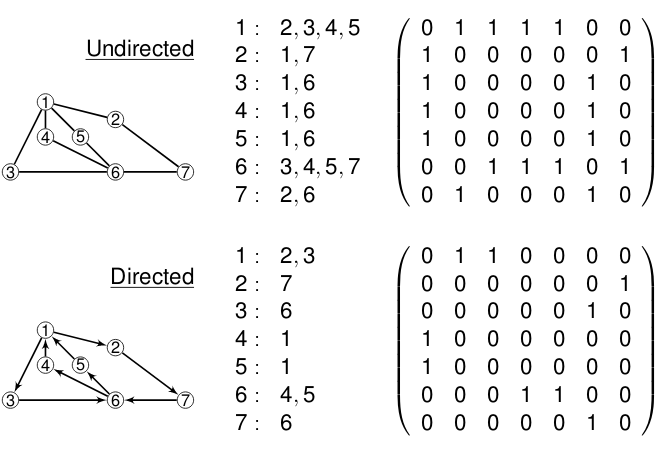
\includegraphics[scale=0.7]{representation}
\end{center}
For each representation:
\begin{itemize}
	\item How much space do we need to store it?
	\item How long does it take to initialize an empty graph?
	\item How long does it take to make a copy?
	\item How long does it take to insert an edge?
	\item How long does it take to list the vertices adjacent to a vertex u?
	\item How long does it take to find out if the edge (u,v) belongs to G?
\end{itemize}
\section{Breadth-First Search}
\begin{itemize}
	\item Input: a graph $G=(V,E)$ and a source vertex s
	\item Aim: to find the distance from s to each of the other vertices in the graph
	\item Idea: send out a \textbf{wave} from s
	\begin{itemize}
		\item The wave first hits vertices at distance 1
		\item Then the wave hits vertices at distance 2
		\item and so on
	\end{itemize}
	\item BFS maintains a queue that contains vertices that have been discovered but are waiting to be processed
	\item BFS colours the vertices:
	\begin{itemize}
		\item White indicates that a vertex is undiscovered
		\item Grey indicates that a vertex is discovered but unprocessed
		\item Black indicates that a vertex has been processed
	\end{itemize}
	\item The algorithm maintains an \textbf{array} d (distance)
	\begin{itemize}
		\item $d[s]=0$ where s is the source vertex
		\item if we discover a new vertex v while processing u, we set $d[v]=d[u]+1$
	\end{itemize}
\end{itemize}
\subsection{Example}
\begin{center}
	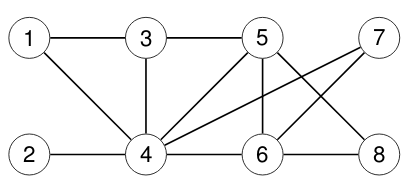
\includegraphics[scale=0.7]{example}
\end{center}
\begin{itemize}
	\item Initialization: source vertex grey, others are while; distance to source is 0; add source to the queue
	\item While the queue is not empty
	\begin{itemize}
		\item Remove first vertex v from the queue
		\item add white neighbours of v to queue and colour them grey; distance is 1 greater than to v
		\item colour v black
	\end{itemize}
\end{itemize}
\subsection{Pseudocode}
\begin{center}
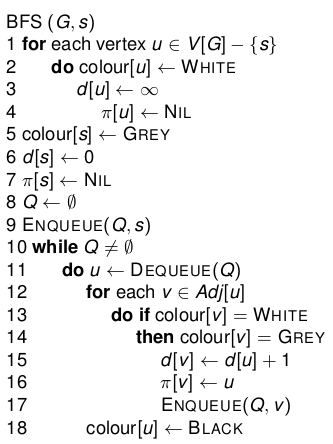
\includegraphics[scale=0.7]{BFS}
\end{center}
\subsection{Analysis of running time}
\begin{itemize}
\item We want an upper bound on the worst case running time
\item Assume that it takes constant time for each operation such as to teat and update colours, to make changes to distance (and predecessor) and to enqueue and dequeue
\item Initialization takes time $\mathcal{O}(V)$
\item Each vertex enters (and leaves) the queue exactly one. So queueing operations take $\mathcal{O}(V)$
\item In the loop the adjacency lists of each vertex are scanned. Each list is read once, and the combined lengths of the lists is $\mathcal{O}(E)$
\item Thus the total running time is $\mathcal{O}(V+E)$
\end{itemize}
\subsection{More than distances}
\begin{itemize}
	\item What if as well as finding the distance to each vertex, we want to be able to find a shortest possible path from the source to each vertex?
	\begin{itemize}
		\item Recursively ask predecessors of nodes until you get back to the start node
		\item BFS used the predecessor of v and v for each vertex v. Note that the predecessor is denoted by $\Pi$
		\item The path from the source S in the Breadth First Tree is a shortest path from S to V 
	\end{itemize}
	
	
	\item What should we add to the algorithm to achieve this?
\end{itemize}
\section{Breadth-first search}
\begin{itemize}
	\item Note that the algorithm runs on both directed and undirected graphs
	\item Notice that the highlighted edges (the ones used to discover new vertices) form a tree: we call this a \textbf{Breadth-first tree}. A path from s to another vertex v through the tree is the shortest path between s and v
	\item The predecessor of a vertex is the one from which is was discovered (i.e. its parent in the Breadth-first tree). We can record predecessors in an array $\Pi$ when we run the algorithm and then use this array to construct the breadth-first tree
\end{itemize}
\end{document}